\begin{figure}[h]\centering
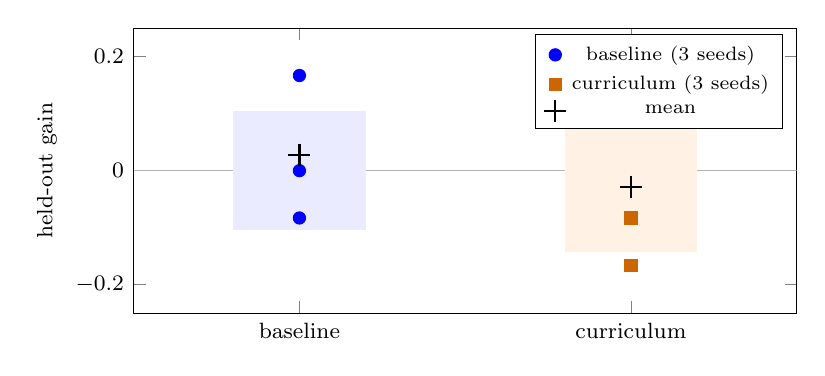
\begin{tikzpicture}
\begin{axis}[width=10cm,height=5.2cm,
  xtick={1,2},xticklabels={baseline,curriculum},xmin=0.5,xmax=2.5,
  ylabel={held-out gain},ymin=-0.25,ymax=0.25,
  tick label style={font=\footnotesize},label style={font=\footnotesize},
  legend style={font=\scriptsize,at={(0.98,0.98)},anchor=north east}]
\draw[black!30] (axis cs:0.5,0)--(axis cs:2.5,0);
% noise band +/- sd
\fill[blue!8] (axis cs:0.8,-0.104)rectangle(axis cs:1.2,0.104);
\fill[orange!10] (axis cs:1.8,-0.142)rectangle(axis cs:2.2,0.142);
\addplot[only marks,mark=*,blue,mark size=2.2pt] coordinates {(1,0.0)(1,0.167)(1,-0.083)};
\addplot[only marks,mark=square*,orange!80!black,mark size=2.2pt] coordinates {(2,0.167)(2,-0.083)(2,-0.167)};
\addplot[mark=+,mark size=4pt,black,thick,only marks] coordinates {(1,0.028)(2,-0.028)};
\legend{baseline (3 seeds),curriculum (3 seeds),mean}
\end{axis}
\end{tikzpicture}
\caption{Multi-seed campaign (real data). Per-seed held-out gains; shaded bands are $\pm 1$ sd. Baseline mean $+0.028$ vs curriculum $-0.028$ (difference $\approx 0.056$, SE $\approx 0.10$, $t\approx0.6$): \emph{no significant difference}, and curriculum costs $\sim$5--6$\times$ the sampling. The single-seed curriculum win ($+0.167$) was noise.}
\end{figure}
